% Szablon pracy dyplomowej. W razie potrzeby można oczywiście dodawać nowe pakiety.

%DIF PREAMBLE EXTENSION ADDED BY LATEXDIFF
%DIF UNDERLINE PREAMBLE
\RequirePackage[normalem]{ulem}
\RequirePackage{color}\definecolor{RED}{rgb}{1,0,0}\definecolor{BLUE}{rgb}{0,0,1}
\providecommand{\DIFadd}[1]{{\protect\color{blue}\uwave{#1}}}
\providecommand{\DIFdel}[1]{{\protect\color{red}\sout{#1}}}
%DIF SAFE PREAMBLE
\providecommand{\DIFaddbegin}{}
\providecommand{\DIFaddend}{}
\providecommand{\DIFdelbegin}{}
\providecommand{\DIFdelend}{}
%DIF FLOATSAFE PREAMBLE
\providecommand{\DIFaddFL}[1]{\DIFadd{#1}}
\providecommand{\DIFdelFL}[1]{\DIFdel{#1}}
\providecommand{\DIFaddbeginFL}{}
\providecommand{\DIFaddendFL}{}
\providecommand{\DIFdelbeginFL}{}
\providecommand{\DIFdelendFL}{}
%DIF END PREAMBLE EXTENSION ADDED BY LATEXDIFF

\pdfoutput=1
\pdfcompresslevel=9
\pdfinfo
{
    /Author ()
    /Title ()
    /Subject ()
    /Keywords ()
}
\documentclass[a4paper,onecolumn,twoside,12pt]{mwrep}

\usepackage{algorithm}
\usepackage{tikz}
\usepackage{hhline}
\usepackage{fixltx2e}
\usetikzlibrary{arrows,shapes}

\usepackage{color}
\usepackage{algpseudocode}
\usepackage{times}
\usepackage[utf8x]{inputenc}
\usepackage[T1]{fontenc}
%\usepackage[polish]{babel}
\usepackage{polski}
\usepackage{setspace}
\usepackage{amsfonts}
\usepackage{amsmath}
\usepackage{array,longtable}
\usepackage{pdflscape}
\usepackage{afterpage}
\usepackage{backref}

\renewcommand*{\backref}[1]{}
\renewcommand*{\backrefalt}[4]{%
    \ifcase #1 (Brak cytowania.)%
    
    \or        (Cytowanie na stronie~#2.)%
    \else      (Cytowanie na stronach~#2.)%
    \fi}
\renewcommand*{\backreftwosep}{ i~}%
\renewcommand*{\backreflastsep}{ i~}%

\hyphenpenalty=10000
\clubpenalty=10000	
\widowpenalty=10000	
\brokenpenalty=10000
\exhyphenpenalty=999999	
\righthyphenmin=3

\newcolumntype{C}{>{\rowfont}c}
\newcommand\setrowfont[1]{\noalign{\gdef\rowfont{#1}}}
\gdef\rowfont{}

\tolerance=4500
\pretolerance=250
\hfuzz=1.5pt
\hbadness=1450

\renewcommand{\labelitemi}{$\bullet$}

\makeatletter
\newcommand{\newalgname}[1]{%
  \renewcommand{\ALG@name}{#1}%
}
\newalgname{Algorytm}
\renewcommand{\listalgorithmname}{Liste des \ALG@name s}
\makeatother

\newcommand*\conj[1]{\bar{#1}}
\newcommand*\mean[1]{\bar{#1}}
\newcommand{\norm}[1]{\left\lVert#1\right\rVert}

\newcommand{\LongComment}[1]{\Comment{\parbox[t]{.45\linewidth} {#1}}}

\sloppy

\setlength{\textwidth}{\paperwidth}
\addtolength{\textwidth}{-5cm}
\setlength{\textheight}{\paperheight}
\addtolength{\textheight}{-5cm}
\setlength{\oddsidemargin}{0.0cm}
\setlength{\evensidemargin}{0.0cm}
\topmargin -1.25cm
\footskip 1.4cm

\linespread{1.5}

\begin{document}

\setcounter{page}{1}
\pagestyle{plain}
\tableofcontents

\chapter{Układ i zawartość pracy}\label{chap:introduction}
Praca inżynierska powinna się składać z czterech rozdziałów. Dwa pierwsze rozdziały zawierają opis dziedziny problemu i opis wykorzystywanych technologii (jedno zagadnienie w każdym z rozdziałów). Dwa kolejne rozdziały stanowią dokumentację techniczną powstałej aplikacji oraz dokumentację użytkownika.

\section{Wstęp}
Wstęp pracy dyplomowej powinien być podzielony na dwie części. Pierwsza część zawiera opis problemu:
\begin{itemize}
\item jaki jest obecny 'stan faktyczny'? 
\item jaki problem dostrzegamy?
\item jakie są istniejące rozwiązania?
\item dlaczego warto się tym zajmować?
\end{itemize}

Następnie wskazuje się \textbf{cel} i \textbf{zakres} pracy. Celem będzie najczęściej rozwiązanie problemu poprzez dostarczenie aplikacji, która wspomaga jakieś działanie. Zakres informuje, co właściwie zostało w ramach pracy zrobione.

W drugiej części wstępu opisuje się zawartość rozdziałów, na przykład w taki sposób:

\emph{
W rozdziale pierwszym niniejszej pracy opisano najważniejsze pojęcia z dziedziny...
Rozdział drugi zawiera opis technologii wykorzystanych w niniejszej pracy.
Dokumentację techniczną powstałej aplikacji MyAwesomeApp przedstawiono w rozdziale 3. W rozdziale 4 zawarto dokumentację użytkownika aplikacji MyAwesomeApp.}

UWAGI:
\begin{itemize}
\item wstęp do pracy piszemy na końcu - dla uniknięcia ciągłych jego przeróbek
\item wstęp powinien mieć ok \textbf{1.5 strony}
\end{itemize}

\section{Opis dziedziny problemu}
W pierwszym rozdziale pracy powinno znaleźć się wprowadzenie w dziedzinę problemu, którego dotyczy praca. Należy opisać na przykład:
\begin{itemize}
\item Postawienie problemu: wprowadzenie do tematu, jak dużo ludzi jest związanych z dziedziną pracy, jak obecnie wyglądają rozwiązania z dziedziny problemu (jakie cechy mają), jakich cech nie mają. W ten sposób dochodzimy do \emph{postawienia problemu}. Potem wskazujemy \emph{pomysł} na rozwiązanie.
\item Szczegółowy opis dziedziny problemu: najważniejsze pojęcia, zasady, reguły itd.
\item Przegląd istniejących rozwiązań: jakie rozwiązania są obecnie na rynku, szczegółowy opis ich funkcjonalności, ceny i wymagania sprzętowe tych rozwiązań, dostępność, rysunki z~działania (o ile da się je zrobić)
\item Podsumowanie - uzasadnienie, dlaczego wybrane do implementacji rozwiązanie jest sensowne i jak poradzi sobie z problemem.
\end{itemize}

UWAGA: Rozdział powinien zawierać kilkuzdaniowe wprowadzenie.

\section{Wykorzystane technologie}
W drugim rozdziale pracy (można zamienić kolejność, jeżeli praca dotyczy technologii a~tworzona aplikacja jest tylko przykładem jej wykorzystania). Należy napisać:
\begin{itemize}
\item Bardzo krótkie streszczenie dotyczące aktualnie dostępnych technologii (np. w zakresie aplikacji internetowych należy wymienić kilka serwerów aplikacji, frameworków do logiki biznesowej i do interfejsu użytkownika). Należy przyjąć pewne założenia pozwalające ograniczyć wybór spośród dużej liczby technologii. Najlepiej oczywiście aby były one sensowne.
\item Szczegółowe przedstawienie technologii konkurencyjnych, np. jeśli piszemy pracę z~dziedziny frameworków Javy do tworzenia aplikacji internetowych, to konkurencją najczęściej będą inne frameworki Javy do tworzenia aplikacji internetowych. Zakres konkurencji wynika z przyjętych wcześniej założeń. Nie należy jednak tworzyć sztucznych ograniczeń aby tylko 'nasza' technologia się nadawała.
\item Szczegółowy opis wybranej technologii. Podrozdział powinien zawierać: opis architektury frameworka, najważniejsze cechy, opis konkstrukcji składniowych (z przykładowym kodem na listingach).
\end{itemize}

% UWAGA: Proszę nie zapominać o wprowadzeniu na początku rozdziału

\section{Dokumentacja techniczna}
Rozdział powinien stanowić opis, w jaki sposób stworzona aplikacja została wykonana. 
Na początku powinien znajdować się \emph{opis założeń}, aby była możliwa późniejsza weryfikacja czy zaproponowana architektura aplikacji 'jest sensowna'. Następne podrozdziały mogą być związane z warstwami (np. dane, logika, widok lub model, kontrolery, widoki). W tym dokumentacji technicznej nie powinno się już dokładać nowych wiadomości z zakresu samej technologii, w której wykonana jest aplikacja - jeżeli taki opis wyda się niezbędny na tym etapie pisania pracy, to należy dodać odpowiednią treść do rozdziału o technologii.

W rozdziale mile widziane są diagramy. Większość diagramów można wygenerować automatem przy pomocy środowiska deweloperskiego. W szczególności:
\begin{itemize}
\item diagram komponentów i wdrożeń, diagramy klas dla poszczególnych warstw
\item diagram sekwencji, stanów, czynności, w zależności od potrzeby
\end{itemize}

W tym rozdziale mile widziane są również listingi pokazujące wykorzystanie wybranych aspektów stosowanej technologii. Nie powinny być one zbyt długie, ani stanowić powielenia 'przykładowych' listingów z rozdziału o technologii.

\section{Dokumentacja użytkownika}
W ostatnim rozdziale pracy należy opisać funkcjonalność dostarczonej aplikacji. Najlepiej posiłkować się w tym miejscu diagramem przypadków użycia. W kolejnych podrozdziałach należy zawrzeć opis typowego scenariusza korzystania ze stworzonej aplikacji. Bardzo mile widziane są rysunki przedstawiające wygląd aplikacji po realizacji kolejnych kroków scenariusza.

\section{Bibliografia i spisy}
Praca powinna zawierać:
\begin{itemize}
\item spis treści na początku
\item bibliografię (na końcu)
\item spis rysunków (na końcu)
\item spis tabel (na końcu)
\item spis listingów (na końcu)
\end{itemize}


\chapter{Uwagi redakcyjne}
\section{Formatowanie tekstu}
Wygodna czcionka do czytania to Times New Roman (12pt), interlinia 1.5. Do wydruku jednostronnego lewy margines powinien być szerszy o ok. 1cm - ułatwi to oprawę pracy. Tekst powinien być wyjustowany a akapit rozpoczynany od wcięcia.

\begin{itemize}
\item Wprowadzane pojęcia piszemy \textbf{pogrubioną} czcionką.

PRZYKŁAD: Chromosomy osobników wchodzących w skład populacji składają się z~\textbf{genów}. Każdy gen przechowuje zakodowaną informację o \dots

\item Wszelkie skróty powinny być wyjaśnione.

PRZYKŁAD: W implementacji projektu MyAwesomeApp wykorzystano metodykę DDD (Domain Driven Design).

\item Pojęcia tłumaczone z języka angielskiego powinny mieć podane w nawiasie oryginalne brzmienie zapisane \textit{kursywą}.

PRZYKŁAD: Wstrzykiwanie zależności (ang. \textit{dependency injection}) jest techniką pozwalającą na odseparowanie komponentów wchodzących w skład aplikacji.

\end{itemize}

Oczywiście powyższe zasady stosujemy wyłącznie w przypadku pierwszego pojawienia się danego pojęcia w tekście.

\section{Tabele, rysunki, listingi, odwołania}

Rysunki i tabele powinny być wycentrowane. Podpisy do rysunków i tabel wstawiamy według poniższego przykładu:

\begin{table}[h]
\begin{center}
\caption{Przykładowe wartości dla funkcji $x^2+y^2$}\label{table:wartosci}
\begin{tabular}{|c|c|c|}
\hline
\textbf{x} & \textbf{y} & \textbf{wartość} \\\hline
0 & 0 & 0 \\\hline
2 & 1 & 5 \\\hline
3 & 3 & 18 \\\hline
\end{tabular}
\end{center}
\end{table}

\begin{figure}[h]\label{fig:miary}
\begin{center}
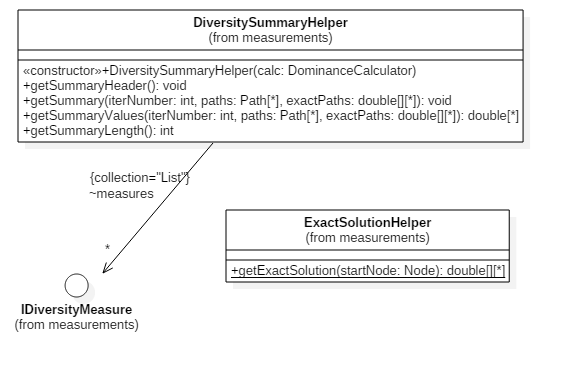
\includegraphics[width=4in]{img/kod/miary2.png}
\caption{Diagram klas dla komponentu [Opracowanie własne]}
\end{center}
\end{figure}

Listingi powinny być numerowane. Kod w listingach powinien być pisany czcionką o~stałej szerokości z zachowaniem wcięć takich jakie stosuje się w IDE do jego pisania. Można usunąć kolorowanie składni, jeżeli przy kopiowaniu ze środowiska developerskiego zostało ono zachowane. Bardzo wygodnie jest, kiedy linie na listingach są numerowane (wtedy można się do nich odwoływać). Najważniejsze linie można pogrubić. 

Podpisy do tabel powinny być wyśrodkowane i położone nad tabelą. Podpisy do rysunków powinny być wyśrodkowanie i położone pod rysunkiem. Poniżej pokazano sposób odwoływania się do tabel i rysunków. Analogicznie odwołujemy się do rozdziałów.

\textit{Przykładowe wartości funkjci $x^2+y^2$ pokazano w tabeli \ref{table:wartosci}.}

\textit{\dots obliczono przykładowe wartości funkcji (Tabela \ref{table:wartosci}).}

\textit{\dots co pokazano na rysunku }

\textit{W rozdziale \ref{chap:introduction} omówiono podstawowe zasady pisania pracy dyplomowej.}

Odwołania do literatury powinny być zrealizowane jak w poniższym przykładzie (wpisy bibliograficzne pod koniec):

Pojęcie optymalizacji wielokryterialnej zostało szczegółowo opisane w pracy \cite{warburton1987approximation}. Dhillon \cite{dhillon2001co} wprowadził pojęcie metod spektralnych podziału grafu. Zagadnienie to jest opisane również w pracach \cite{DBLP:conf/icaisc/2012-2, guo2008regionalization}.

\section{Forma wypowiedzi w pracy}
\begin{itemize}
\item Praca powinna być napisana w formie bezosobowej, na przykład: '\textit{uzyskane wyniki pokazują, że}' zamiast '\textit{uzyskałam/em wyniki, które pokazują, że}' lub '\textit{opracowana aplikacja}' zamiast '\textit{moja aplikacja}' 
\item Do rozdziałów/rysunków/tabel odwołujemy się przy pomocy numerów a nie słów 'powyżej', 'poniżej', 'w poprzednim rozdziale'.
\item Pisząc o samej pracy używamy zwrotu 'niniejsza praca', bieżący rozdział to 'niniejszy rozdział'
\item Nie korzystamy ze skrótów, takich jak \emph{np., nr, itd.}
\item Staramy się pisać możliwie krótkimi zdaniami - zdania wielokrotnie złożone są bardzo trudne do czytania.
\item W czasie pisania nie zmieniamy czasu, strony ani trybu czasownika. Szczególnie razi to w następujących po sobie zdaniach.
\item Każdy rozdział zaczynamy kilkoma zdaniami wprowadzenia - \emph{'W niniejszym rozdziale zaprezentowano zbiór najważniejszych pojęć z dziedziny \dots. W kolejnych podrozdziałach omówiono \dots'}
\item Każdy rozdział kończymy kilkoma zdaniami podsumowania/wniosków
\end{itemize}

\section{Edycja tekstu w \LaTeX}
Gorąco zachęcam do składania pracy w \LaTeX. Ma to cały zestaw zalet:
\begin{itemize}
\item Bardzo trudno jest złożyć pracę brzydko.
\item Wszelkie odwołania realizowane są półautomatycznie.
\item Praca ze środowiskiem do \LaTeX-a bardzo przypomina pracę z edytorem tekstu, może za wyjątkiem tego, że nie trzeba co chwilę odrywać rąk od klawiatury i wybierać czegoś z~menu.
\item Składnia jest bardzo prosta - na użytek pracy inżynierskiej potrzebna jest znajomość co najwyżej kilku komend.
\item Jest gotowy szablon do pracy
\item Tekst pracy można wersjonować
\end{itemize}

Aby edycja tekstu była łatwiejsza i przyjemniejsza polecam korzystanie z narzędzia \textbf{TeXstudio} i dystrybucji \textbf{TeXlive}.
\bibliographystyle{plain}
\bibliography{sample.bib}
\listoffigures
\listoftables
\end{document}